To show the efficacy of our method, we consider the two test cases outlined in Section~\ref{sec:application-to-the-helmholtz-equation}.
In these, we set $r_{in}\equiv\frac{1}{4}$, $r_{out}=1$, and the mollifier radius $r_{mol}=0.9 < r_{out}$ and use the linear exterior mollifier~\eqref{eq:exterior_mollifier}.
Hence, we have $\diam(D)=2$ and $\left\| \nabla \chi(\x) \right\|_{L^{\infty}}=\frac{1}{r_{mol} - r_{in}}$.
We initialize with a mean-based preconditioner at $\yb=\bm{0}\in\mathbb{R}^N$ and test our routine by considering $|W|=1000$ points, randomly selected and uniformly distributed in $Y=[-1,1]^N$.
The~1000 parameter locations are fixed per parameter dimension throughout the numerical experiments.

We have implemented the numerical methods in Python~3.10, running in an Ubuntu~$22.04$ Docker container.
To obtain the linear systems, we meshed our computational domain using Gmsh~\cite{geuzaine2009} with uniform mesh size $h\sim k^{-\frac{3}{2}}$ to counteract the pollution effect~\cite{babuska1997}.
We use DOLFINx~\cite{alnaes2014a,baratta2023,scroggs2022,scroggs2022a} to construct the linear systems, which we solve with GMRES in PETSc~\cite{brown2022} until the default relative error ($10^{-5}$).
Moreover, we construct the required preconditioners using PETSc as well.
GMRES iterations and PETSc preconditioner construction have been timed using the \texttt{time.process\_time()} method of the \texttt{time} module in Python.
We perform the optimization during the location-allocation steps using the L-BFGS-B Fortran subroutine.
When timing pieces of code, we exclude any overhead caused by the assembly of the linear systems~\eqref{eq:linear_system} because we need to assemble them anyway, independently of the preconditioning strategy.

We will first focus on the parameterized shape problem in Section~\ref{subsec:conventional_comparison}, as these results give more insight into the efficacy of the algorithm.
Subsequently, in Section~\ref{subsec:algorithm-performance-for-the-affine-expansion}, we will use the affine case to discuss the effects of isotropy in the parameter domain and to see a practical example of the concentration of measure effect discussed in Remark~\ref{rem:high-dimensional-parameter-space}.
In Sections~\ref{subsec:preconditioner-placement}--\ref{subsec:kernel-comparison}, we show further numerical studies on the performance and accuracy of Algorithms~\ref{alg:location-allocation} and~\ref{alg:gray-box-gpr}.

Except for the high-frequency results in Table~\ref{tab:k120}, all computations have been performed five times and have been averaged to reduce randomness effects.

\subsection{Algorithm performance for the parameterized domain}\label{subsec:conventional_comparison}
We demonstrate the improvements of distributed preconditioning over more traditional approaches, such as mean-based preconditioning, using parameter dimensions ranging from $N=2$ to $N=25$.

For each experiment, we report the time to train the gray-box GPR ($t_{train}$), the location-allocation time ($t_{l-al}$), and the execution time ($t_{exec}$) of solving the preconditioned linear systems, rounded to the nearest second, and averaged over several runs to reduce the variance.
Moreover, we list the average number of GMRES iterations in the executed strategy ($it_{av}$).
The total computation time ($t_{tot}=t_{train} + t_{l-al}+t_{exec}$) follows.
Additionally, we list the average number of placed preconditioners $N_{pc}$ over the runs.

\subsubsection{Fixed shape variations and anisotropy}
Table~\ref{tab:alltestdata} shows various results for the shape problem.
In Table~\ref{tab:midtheta}, we find the results for a medium value for the shape variation parameter $\vartheta$ and a low value for the anisotropy parameter $\alpha$, and we can see that the dimensionality of the problem has a significant effect on the algorithm performance.
As expected, the gray-box GPR takes longer to train as the parameter dimension increases.
Additionally, $t_{l-al}$ increases rapidly with the parameter dimension, and this increase is more pronounced than in the training time.
This is because the GPR training accounts for parameter dimension anisotropy via the Gaussian process correlation lengths, while the location-allocation does not.
On the other hand, the number of preconditioners placed is relatively stable across parameter dimensions.

Finally, when we compute the total computation time $t_{tot}=t_{train} + t_{l-al} + t_{exec}$, we observe that it ranges from $8,000$ to $14,000$ seconds, increasing with the parameter dimension.
In these experiments, a single LU preconditioner takes around $t_{pc}=75$ seconds, leading to a baseline computation time of $|W|\times t_{pc}=75,000$ seconds when not using a preconditioning strategy, significantly more than the observed range for $t_{tot}$.
Therefore, we have realized a significant reduction in the total computation time.
A single mean-based preconditioner does not work very well in this case, as the number of GMRES iterations rises sharply as $\left| \y \right|$ increases, for which we do not compare against it.
We note that we only know this rises sharply because we have trained the surrogate $m(\cdot)$; it is not clear a-priori whether this is the case or not.
We observed values for $m_{\max}$ in equation~\eqref{eq:f-acq-def} of around $100$ throughout these and other experiments.

\subsubsection{Varying the amount of shape variations}
In Table~\ref{tab:hightheta}, the maximal shape variation parameter $\vartheta$ is double from the baseline, just large enough that no self-intersecting curves can occur.
In contrast, Table~\ref{tab:lowtheta} shows the case when the maximal shape variation is halved with respect to the baseline, resulting in significantly smaller shape variations.
This affects matrix values but preserves the overall structure in the parameter dependence.

Through these experiments, we observe that increasing $\vartheta$ increases training time while reducing $\vartheta$ decreases it.
For $\vartheta = \frac{1}{4}\vartheta_{\max}(\alpha=2)$, we observe the same behavior in the training time with respect to the parameter dimension: larger parameter dimensions require more training time.
The effect of the parameter dimension is lower in the case of smaller $\vartheta$, as fewer training points are needed to satisfy the stopping criterion.
For $\vartheta = \vartheta_{\max}(\alpha=2)$, we observe similar behavior of $N$ as we did for $\vartheta=\frac{1}{2}\vartheta_{\max}(\alpha=2)$, where the training time grows rapidly with the parameter dimension.

The number of preconditioners increases with $\vartheta$, as $m(\y-\yh)$ grows faster with $|\y-\yh|$.
Since $t_{pc}$ and $t_{GMRES}$, and therefore, by equation~\eqref{eq:Nratio}, $N_{ratio}$, are independent of $\vartheta$.
Therefore, the `radius of influence' of a preconditioner is reduced, and the preconditioners will need to be packed more densely.

The total computation time is mainly determined by the execution time $t_{exec}$, which increases for larger $\vartheta$.
This is partly due to the different number of preconditioners and partly due to the slightly larger number of Krylov iterations required as a consequence of the larger variations in the resulting matrices.

\subsubsection{Increased anisotropy}
To study the effects of dimension anisotropy, we modify the decay parameter $\alpha$ in Table~\ref{tab:alpha3}.
Increasing $\alpha$ has two effects: on the one hand, it decreases the importance of higher parameter dimensions, see equation~\eqref{eq:shapew1infnormdef}.
On the other hand, since $\vartheta_{\max}(\alpha=3) > \vartheta_{\max}(\alpha=2)$, it increases the total shape variation parameter $\vartheta$, which we have put to represent total shape variations of the same magnitude.

Foremost, we observe that the values of $t_{train}$ are larger than the values for $\alpha=2$ due to the larger value for $\vartheta$.
On the other side, we see that the training time does not increase much for larger parameter dimensions, clearly showing the effects of the faster decay in the parameter dimension importance.
By contrast, the location-allocation cost $t_{l-al}$ still rises sharply since it does not account for anisotropy.


\begin{table}
    \centering
    \subfloat[][$\vartheta=\vartheta_{\max}(\alpha=2)$, $\alpha=2$.]{
        \begin{tabular}{r|l|l|l|l|l|l}
            $N$&$t_{train}(s)$&$t_{l-al}(s)$&$t_{exec}(s)$&$t_{tot}(s)$&$N_{pc}$&$it_{av}$\\\hline
            2 & 769 & 9 & 10,355 & 11,133 & 44 & 8\\
            5 & 2,161 & 145 & 16,577 & 18,883 & 65 & 14\\
            10 & 4,208 & 1,093 & 18,111 & 23,412 & 69 & 16\\
            15 & 3,416 & 1,514 & 18,602 & 23,532 & 63 & 16\\
            20 & 3,605 & 2,994 & 18,803 & 25,402 & 75 & 16\\
            25 & 5,792 & 5,872 & 19,281 & 30,945 & 67 & 17\\
        \end{tabular}
        \label{tab:hightheta}
    }\\\vspace{20pt}
    \subfloat[][$\vartheta=2^{-1}\vartheta_{\max}(\alpha=2)$, $\alpha=2$.]{
        \begin{tabular}{r|l|l|l|l|l|l}
            $N$&$t_{train}(s)$&$t_{l-al}(s)$&$t_{exec}(s)$&$t_{tot}(s)$&$N_{pc}$&$it_{av}$\\\hline
            2 & 402 & 6 & 7,254 & 7,662 & 34 & 6\\
            5 & 515 & 51 & 9,165 & 9,731 & 34 & 9\\
            10 & 598 & 167 & 9,287 & 10,052 & 31 & 10\\
            15 & 566 & 393 & 9,517 & 10,476 & 31 & 10\\
            20 & 635 & 588 & 9,302 & 10,525 & 28 & 11\\
            25 & 555 & 943 & 9,693 & 11,191 & 29 & 11\\
        \end{tabular}
        \label{tab:midtheta}
    }\\\vspace{20pt}
    \subfloat[][$\vartheta=2^{-2}\vartheta_{\max}(\alpha=2)$, $\alpha=2$.]{
        \begin{tabular}{r|l|l|l|l|l|l}
            $N$&$t_{train}(s)$&$t_{l-al}(s)$&$t_{exec}(s)$&$t_{tot}(s)$&$N_{pc}$&$it_{av}$\\\hline
            2 & 206 & 4 & 5,877 & 6,087 & 19 & 5\\
            5 & 204 & 22 & 7,101 & 7,327 & 20 & 7\\
            10 & 215 & 85 & 7,124 & 7,424 & 19 & 7\\
            15 & 210 & 137 & 7,099 & 7,446 & 17 & 7\\
            20 & 233 & 238 & 7,063 & 7,534 & 18 & 7\\
            25 & 237 & 408 & 7,203 & 7,848 & 15 & 8\\
        \end{tabular}
        \label{tab:lowtheta}
    }\\\vspace{20pt}
    \subfloat[][$\vartheta=2^{-1}\vartheta_{\max}(\alpha=3)$, $\alpha=3$.]{
        \begin{tabular}{r|l|l|l|l|l|l}
            $N$&$t_{train}(s)$&$t_{l-al}(s)$&$t_{exec}(s)$&$t_{tot}(s)$&$N_{pc}$&$it_{av}$\\\hline
            2 & 452 & 6 & 6,996 & 7,454 & 31&6\\
            5 & 483 & 32 & 8,045 & 8,560 & 29&8\\
            10 & 471 & 127 & 8,059 & 8,657 & 30&9\\
            15 & 447 & 218 & 8,232 & 8,897 & 31&8\\
            20 & 463 & 373 & 7,808 & 8,645 & 29&8\\
            25 & 497 & 606 & 8,183 & 9,285 & 30&8\\
        \end{tabular}
        \label{tab:alpha3}
    }
    \caption{Results of running Algorithms~\ref{alg:location-allocation} and~\ref{alg:gray-box-gpr} with the shape problem introduced in Section~\ref{subsec:parameterized-domain} with a wavenumber $k=60$. Times in seconds and averaged over five runs.}
    \label{tab:alltestdata}
\end{table}

\subsubsection{Lower and higher frequency}
To change problem conditioning and matrix sizes, we modify the frequency $k$ of the Helmholtz equation, with results shown in Table~\ref{tab:shapefrequencies}.
We consider two cases: a lower frequency of $k=30$ and a higher frequency of $k=120$.
To compare the numerical performance, we maintain the size of $W$ at 1000 points.
However, we emphasize that when one is interested in the error in a surrogate or an average using Monte Carlo or sparse grid methods, the number of parameter locations should be adjusted with $k$~\cite{hiptmair2024}.
Due to computational limits, we run our algorithm once for $k=120$ without averaging over multiple runs.

We observe a large difference in the overall magnitude of the computation times: a low value for $k$ corresponds to low computation times and vice versa in the high-frequency case.
In the case $k=30$, we compare the total computation times with the baseline $|W|\times t_{pc}\approx 1000\times 1.5=1500$ seconds and conclude that we have improved the computational load, but barely when the parameter dimension is large.
In the case $k=120$, we have $|W|\times t_{pc}\approx 1000\times 1000s=1,000,000s\approx11.5\text{ days}$, implying we have improved the computational load by a factor of 10.

In the case $k=30$, the location-allocation cost does not increase as much as in the case $k=60$ (Table~\ref{tab:midtheta}).
However, the number of preconditioners is roughly the same as the dimension increases.
This is in contrast to the case $k=120$, where $t_{l-al}$ increases significantly.
We have observed similar increases in Table~\ref{tab:alltestdata}, where the increase can be attributed to the higher number of placed preconditioners.
In this case, the values for $N_{pc}$ are similar, and the increase is due to additional location allocation steps.

The algorithm runs until no further improvements are found or the iteration costs exceed the improvement gained.
Higher computation times allow for more resources to be allocated to location-allocation iterations, which explains the larger values for $t_{l-al}$.
The lower values of $t_{l-al}$ in the $k=30$ case can be explained similarly.
Finally, the number of preconditioners is higher for $k=30$, which is because $\tau_{pc}$ decreases faster than $\tau_{Krylov}$ as the matrix dimension shrinks.

\begin{table}
    \centering
    \subfloat[][$k=30$, $\alpha=2$.]{
        \begin{tabular}{r|l|l|l|l|l|l}
            $N$&$t_{train}(s)$&$t_{l-al}(s)$&$t_{exec}(s)$&$t_{tot}(s)$&$N_{pc}$&$it_{av}$\\\hline
            2 & 14 & 7 & 243 & 264 & 49 & 4\\
            5 & 14 & 40 & 339 & 393 & 60 & 6\\
            10 & 20 & 125 & 362 & 507 & 57 & 7\\
            15 & 20 & 224 & 359 & 604 & 48 & 7\\
            20 & 36 & 254 & 346 & 636 & 30 & 7\\
            25 & 31 & 349 & 349 & 729 & 26 & 8\\
        \end{tabular}
        \label{tab:k30}
    }\\\vspace{20pt}
    \subfloat[][$k=120$, $\alpha=2$.]{
        \begin{tabular}{r|l|l|l|l|l|l}
            $N$&$t_{train}(s)$&$t_{l-al}(s)$&$t_{exec}(s)$&$t_{tot}(s)$&$N_{pc}$&$it_{av}$\\\hline
            2 & 3,291 & 6 & 46,364 & 49,661 & 23 & 9\\
            5 & 10,848 & 60 & 71,575 & 82,484 & 26 & 17\\
            10 & 22,079 & 458 & 81,134 & 103,671 & 24 & 20\\
            15 & 29,513 & 1,169 & 77,540 & 108,222 & 22 & 19\\
            20 & 21,833 & 1,676 & 77,496 & 101,005 & 18 & 22\\
            25 & 31,626 & 3,010 & 77,043 & 111,680 & 22 & 21\\
        \end{tabular}
        \label{tab:k120}
    }
    \caption{Test results for the shape expansion with $\alpha=2$, $\vartheta=2^{-1}\vartheta_{\max}(\alpha=2)$ and varying frequencies. Times in seconds and averaged over five runs.}
    \label{tab:shapefrequencies}
\end{table}

\subsubsection{Number of parameter locations}
Finally, we compare the algorithm performance with different numbers of parameter locations $N_{\text{loc}}=|W|$ for $\alpha=2$, maximal shape variations $\vartheta=\frac{1}{2}\vartheta_{\max}(\alpha=2)$, and frequency $k=60$.
Through this experiment, we can observe the effects of sample density in the parameter space on algorithm performance.


In Figure~\ref{fig:costvsncol}, we have plotted the realized reduction in computation time with respect to using new preconditioners for all parameter locations against the number of parameter locations $N_{\text{loc}}$.
From this figure, we can see that the algorithm realizes more savings for larger $N_{\text{loc}}$
This effect can be explained by considering the cardinality of the training set, which remains relatively constant as $N_{\text{loc}}$ increases.

In Figure~\ref{fig:ncolvsnpc}, we show the number of preconditioners compared to $N_{\text{loc}}$.
The general trend is upwards, implying that more preconditioners are placed as $N_{\text{loc}}$ increases.
However, the rate at which this is happening in Figure~\ref{fig:ncolvsnpc} is less than one, which means that the number of parameter locations allocated to each preconditioner increases as well, as one would expect.

\begin{figure}
    \centering
    \begin{tikzpicture}
        \begin{axis}[
            ymin=65,
            ymax=100,
            xmin=100,
            xmax=9000,
            xmode=log,
            width=0.95\textwidth,
            height=0.5\textwidth,
            ylabel=Savings ($\%$),
            xlabel=Size of $W$,
            ylabel style={font=\small},
            ylabel near ticks,
            legend columns=2,
            transpose legend,
            grid=both,
            legend pos=south east,
            xtick={125, 250, 500, 1000, 2000, 4000, 8000},
            xticklabels={125, 250, 500, 1000, 2000, 4000, 8000},
        ]
            \addplot[viridis_1,thick] table [mark=none, x=ncol, y=d_2]{6-chapter/data/N_col_test/savings.dat};
            \addlegendentry{$N\eq 2$}
            \addplot[viridis_2,thick] table [mark=none, x=ncol, y=d_5]{6-chapter/data/N_col_test/savings.dat};
            \addlegendentry{$N\eq 5$}
            \addplot[viridis_3,thick] table [mark=none, x=ncol, y=d_10]{6-chapter/data/N_col_test/savings.dat};
            \addlegendentry{$N\eq 10$}
            \addplot[viridis_4,thick] table [mark=none, x=ncol, y=d_15]{6-chapter/data/N_col_test/savings.dat};
            \addlegendentry{$N\eq 15$}
            \addplot[viridis_5,thick] table [mark=none, x=ncol, y=d_20]{6-chapter/data/N_col_test/savings.dat};
            \addlegendentry{$N\eq 20$}
            \addplot[viridis_6,thick] table [mark=none, x=ncol, y=d_25]{6-chapter/data/N_col_test/savings.dat};
            \addlegendentry{$N\eq 25$}
        \end{axis}
    \end{tikzpicture}
    \caption{Computational cost savings compared to the size of the parameter set $W$ for the shape expansion with anistropy parameter $\alpha=2$ and shape variations $\vartheta=\frac{1}{2}\vartheta_{\max}(\alpha=2)$.}
    \label{fig:costvsncol}
\end{figure}

\begin{figure}
    \centering
    \begin{tikzpicture}
        \begin{axis}[
            ymin=0,
            ymax=120,
            xmin=100,
            xmax=9000,
            xmode=log,
            grid=both,
            ymode=log,
            width=0.95\textwidth,
            height=0.5\textwidth,
            ylabel=$N_{pc}$,
            xlabel=Size of $W$,
            ylabel style={font=\small},
            ylabel near ticks,
            legend columns=2,
            transpose legend,
            legend pos=north west,
            xtick={125, 250, 500, 1000, 2000, 4000, 8000},
            xticklabels={125, 250, 500, 1000, 2000, 4000, 8000},
        ]
            \addplot[viridis_1,thick] table [mark=none, x=ncol, y=d_2]{6-chapter/data/N_col_test/npc.dat};
            \addlegendentry{$N\eq 2$}
            \addplot[viridis_2,thick] table [mark=none, x=ncol, y=d_5]{6-chapter/data/N_col_test/npc.dat};
            \addlegendentry{$N\eq 5$}
            \addplot[viridis_3,thick] table [mark=none, x=ncol, y=d_10]{6-chapter/data/N_col_test/npc.dat};
            \addlegendentry{$N\eq 10$}
            \addplot[viridis_4,thick] table [mark=none, x=ncol, y=d_15]{6-chapter/data/N_col_test/npc.dat};
            \addlegendentry{$N\eq 15$}
            \addplot[viridis_5,thick] table [mark=none, x=ncol, y=d_20]{6-chapter/data/N_col_test/npc.dat};
            \addlegendentry{$N\eq 20$}
            \addplot[viridis_6,thick] table [mark=none, x=ncol, y=d_25]{6-chapter/data/N_col_test/npc.dat};
            \addlegendentry{$N\eq 25$}
        \end{axis}
    \end{tikzpicture}
    \caption{Number of preconditioners placed compared to the size of the parameter set $W$.}
    \label{fig:ncolvsnpc}
\end{figure}


\subsection{Algorithm performance for the affine expansion}\label{subsec:algorithm-performance-for-the-affine-expansion}
Table~\ref{tab:eta025} shows results for the case of affine expansion outlined in Section~\ref{subsec:disjoint-density}, with a fully isotropic parameter domain, namely $\eta_i=\frac{1}{4}$, for $i=1,\ldots, N$.
This case helps us to study the effects of the parameter anisotropy.

The most obvious effect is shown in the column $N_{pc}$ with only one preconditioner for higher parameter dimensions.
This is due to the concentration effect (Remark~\ref{rem:high-dimensional-parameter-space}) and is in stark contrast to the anisotropic cases discussed before.
Thus, we are using mean-based preconditioning, with an additional training overhead $t_{train}$.

Additionally, the training time $t_{train}$ is not significantly impacted by the parameter dimension.
This is because the prior mean approximates the surrogate very well, requiring only a small number of training points.
To examine this further, we approximate the root-mean-square error (RMSE) for $N=2,10,25$ during training.
Figure~\ref{fig:pietrain} shows that the GPR trains fairly well in the lower dimensional limit, decreasing the RMSE from 10 to 6 quickly, after which the training stagnates.
For high dimensions ($N=25$), the prior fits the model very well, but training does not improve the surrogate.
This highlights the curse of dimensionality, showing that parameter anisotropy is necessary for optimal performance.
\begin{table}
    \centering
    \begin{tabular}{r|l|l|l|l|l|l}
        $N$&$t_{train}(s)$&$t_{l-al}(s)$&$t_{exec}(s)$&$t_{tot}(s)$&$N_{pc}$&$it_{av}$\\\hline
        2 & 1,551 & 3 & 5,339 & 6,884 & 12 & 5 \\
        5 & 1,517 & 11 & 7,329 & 8,909 & 7 & 9 \\
        10 & 1,756 & 0 & 7,167 & 9,011 & 1 & 10 \\
        15 & 1,627 & 0 & 7,501 & 9,203 & 1 & 9 \\
        20 & 1,616 & 0 & 7,383 & 9,091 & 1 & 9 \\
        25 & 1,756 & 0 & 7,168 & 9,011 & 1 & 9 \\
    \end{tabular}
    \captionof{table}{Tabulated results in seconds for affine expansion with $\eta_i=\frac{1}{4}$, $i=n,\ldots, N$.}
    \label{tab:eta025}
\end{table}
\begin{figure}
    \begin{tikzpicture}
        \begin{axis}[
            ymin=0,
            ymax=10,
            xmin=0,
            xmax=200,
            width=0.95\textwidth,
            height=0.4\textwidth,
            ylabel=RMSE,
            ylabel style={font=\small},
            ylabel near ticks,
            legend columns=3,
            transpose legend,
            legend pos=north east,
        ]
            \addplot[viridis_1,thick] table [mark=none, x=iter, y=d2]{6-chapter/data/pietrain025.dat};
            \addlegendentry{$N\eq 2$}
            \addplot[viridis_2,thick] table [mark=none, x=iter, y=d5]{6-chapter/data/pietrain025.dat};
            \addlegendentry{$N\eq 5$}
            \addplot[viridis_3,thick] table [mark=none, x=iter, y=d10]{6-chapter/data/pietrain025.dat};
            \addlegendentry{$N\eq 10$}
            \addplot[viridis_4,thick] table [mark=none, x=iter, y=d15]{6-chapter/data/pietrain025.dat};
            \addlegendentry{$N\eq 15$}
            \addplot[viridis_5,thick] table [mark=none, x=iter, y=d20]{6-chapter/data/pietrain025.dat};
            \addlegendentry{$N\eq 20$}
            \addplot[viridis_6,thick] table [mark=none, x=iter, y=d25]{6-chapter/data/pietrain025.dat};
            \addlegendentry{$N\eq 25$}
        \end{axis}
    \end{tikzpicture}
    \caption{Training RMSE for affine expansion.}
    \label{fig:pietrain}
\end{figure}



\subsection{Preconditioner placement}\label{subsec:preconditioner-placement}
We analyze the efficacy of Algorithm~\ref{alg:location-allocation} in placing the preconditioners, as shown in Figure~\ref{fig:voronoi_diagram}.
To make this insightful, we use a low parameter dimension of $N=2$, which allows for clear visualizations, and we sample uniformly over the parameter space.
Figure~\ref{fig:1a} shows the result of the location-allocation algorithm.
The colored dots represent the parameter values grouped by their assigned preconditioner indicated by color.
Moreover, in black, the borders of the generalized Voronoi diagram are shown.

From Figure~\ref{fig:voronoi_diagram}, it is clear that the edges of the Voronoi diagram are curved because the Voronoi distance is based on $m(\cdot)$ shown in Figure~\ref{fig:1b}, which deviates from the actual distance to the preconditioner.
Moreover, Figure~\ref{fig:1a} shows that not all preconditioners are placed at parameter locations; see Remark~\ref{rem:pcnotatcol}.


\begin{figure}
    \centering
    \begin{subfigure}{0.50\textwidth}
        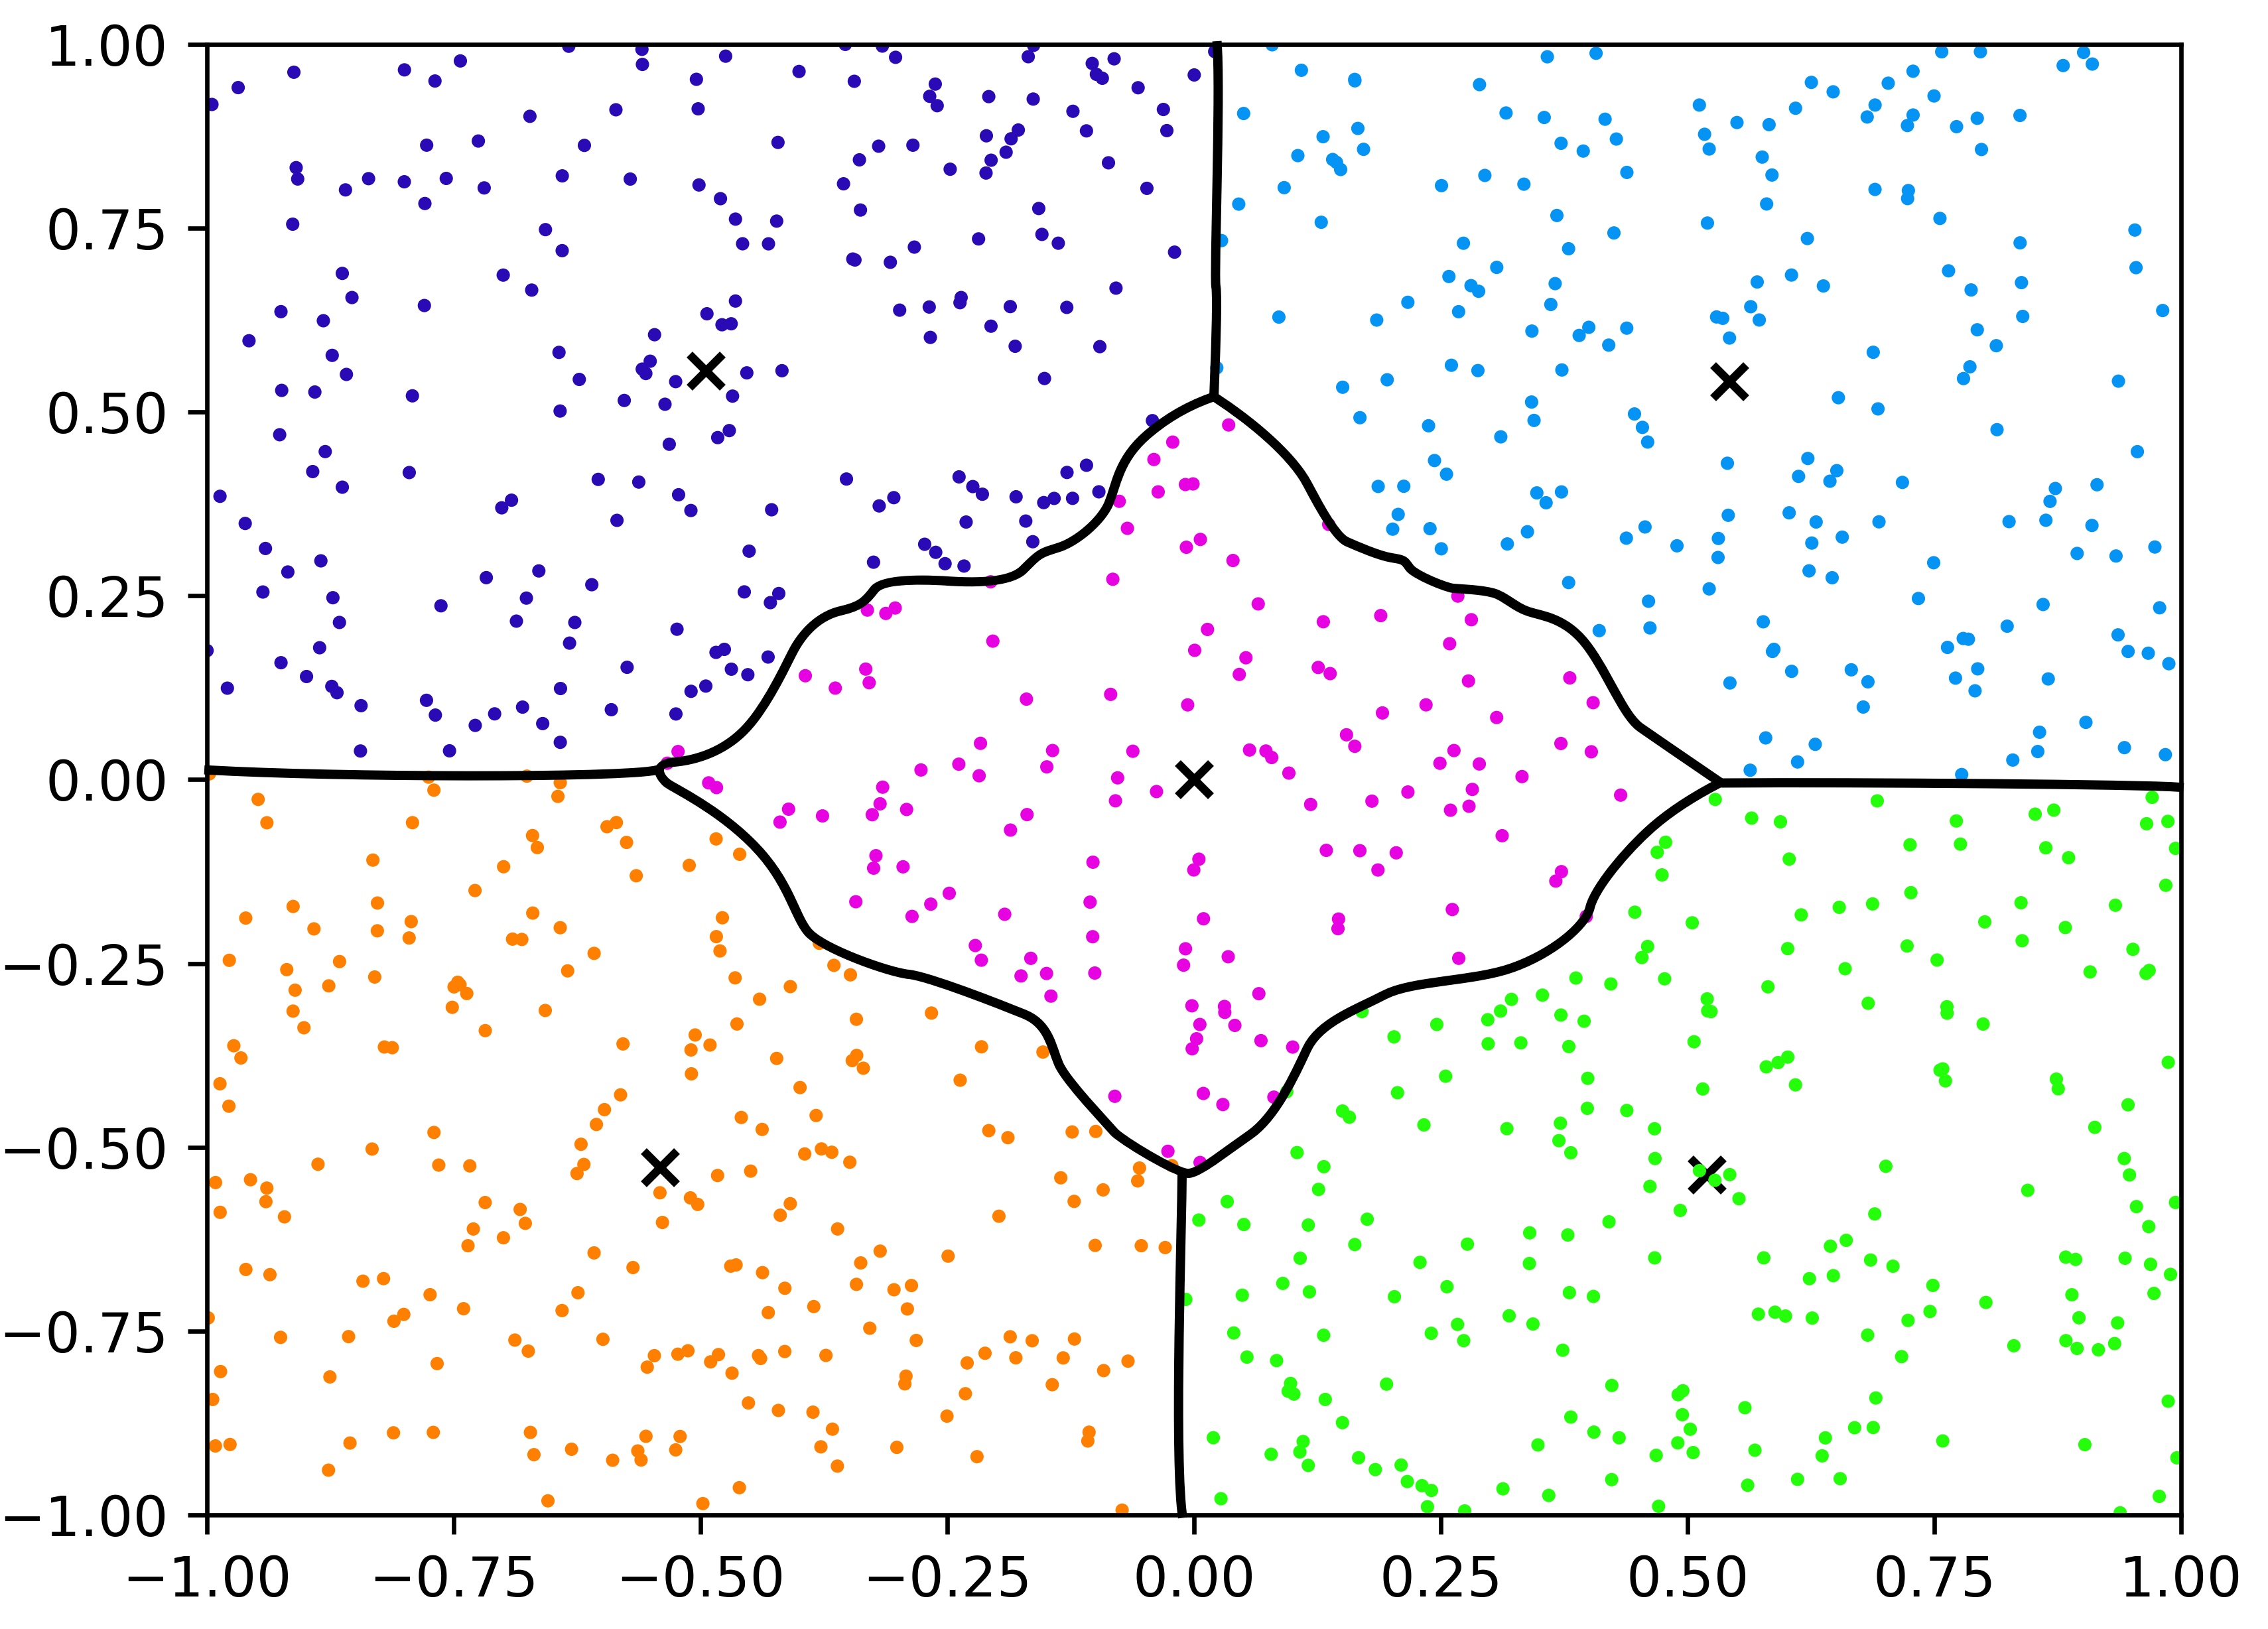
\includegraphics[width=\linewidth]{6-chapter/figures/vor_lines2}
        \caption{} \label{fig:1a}
    \end{subfigure}%
    \begin{subfigure}{0.50\textwidth}
        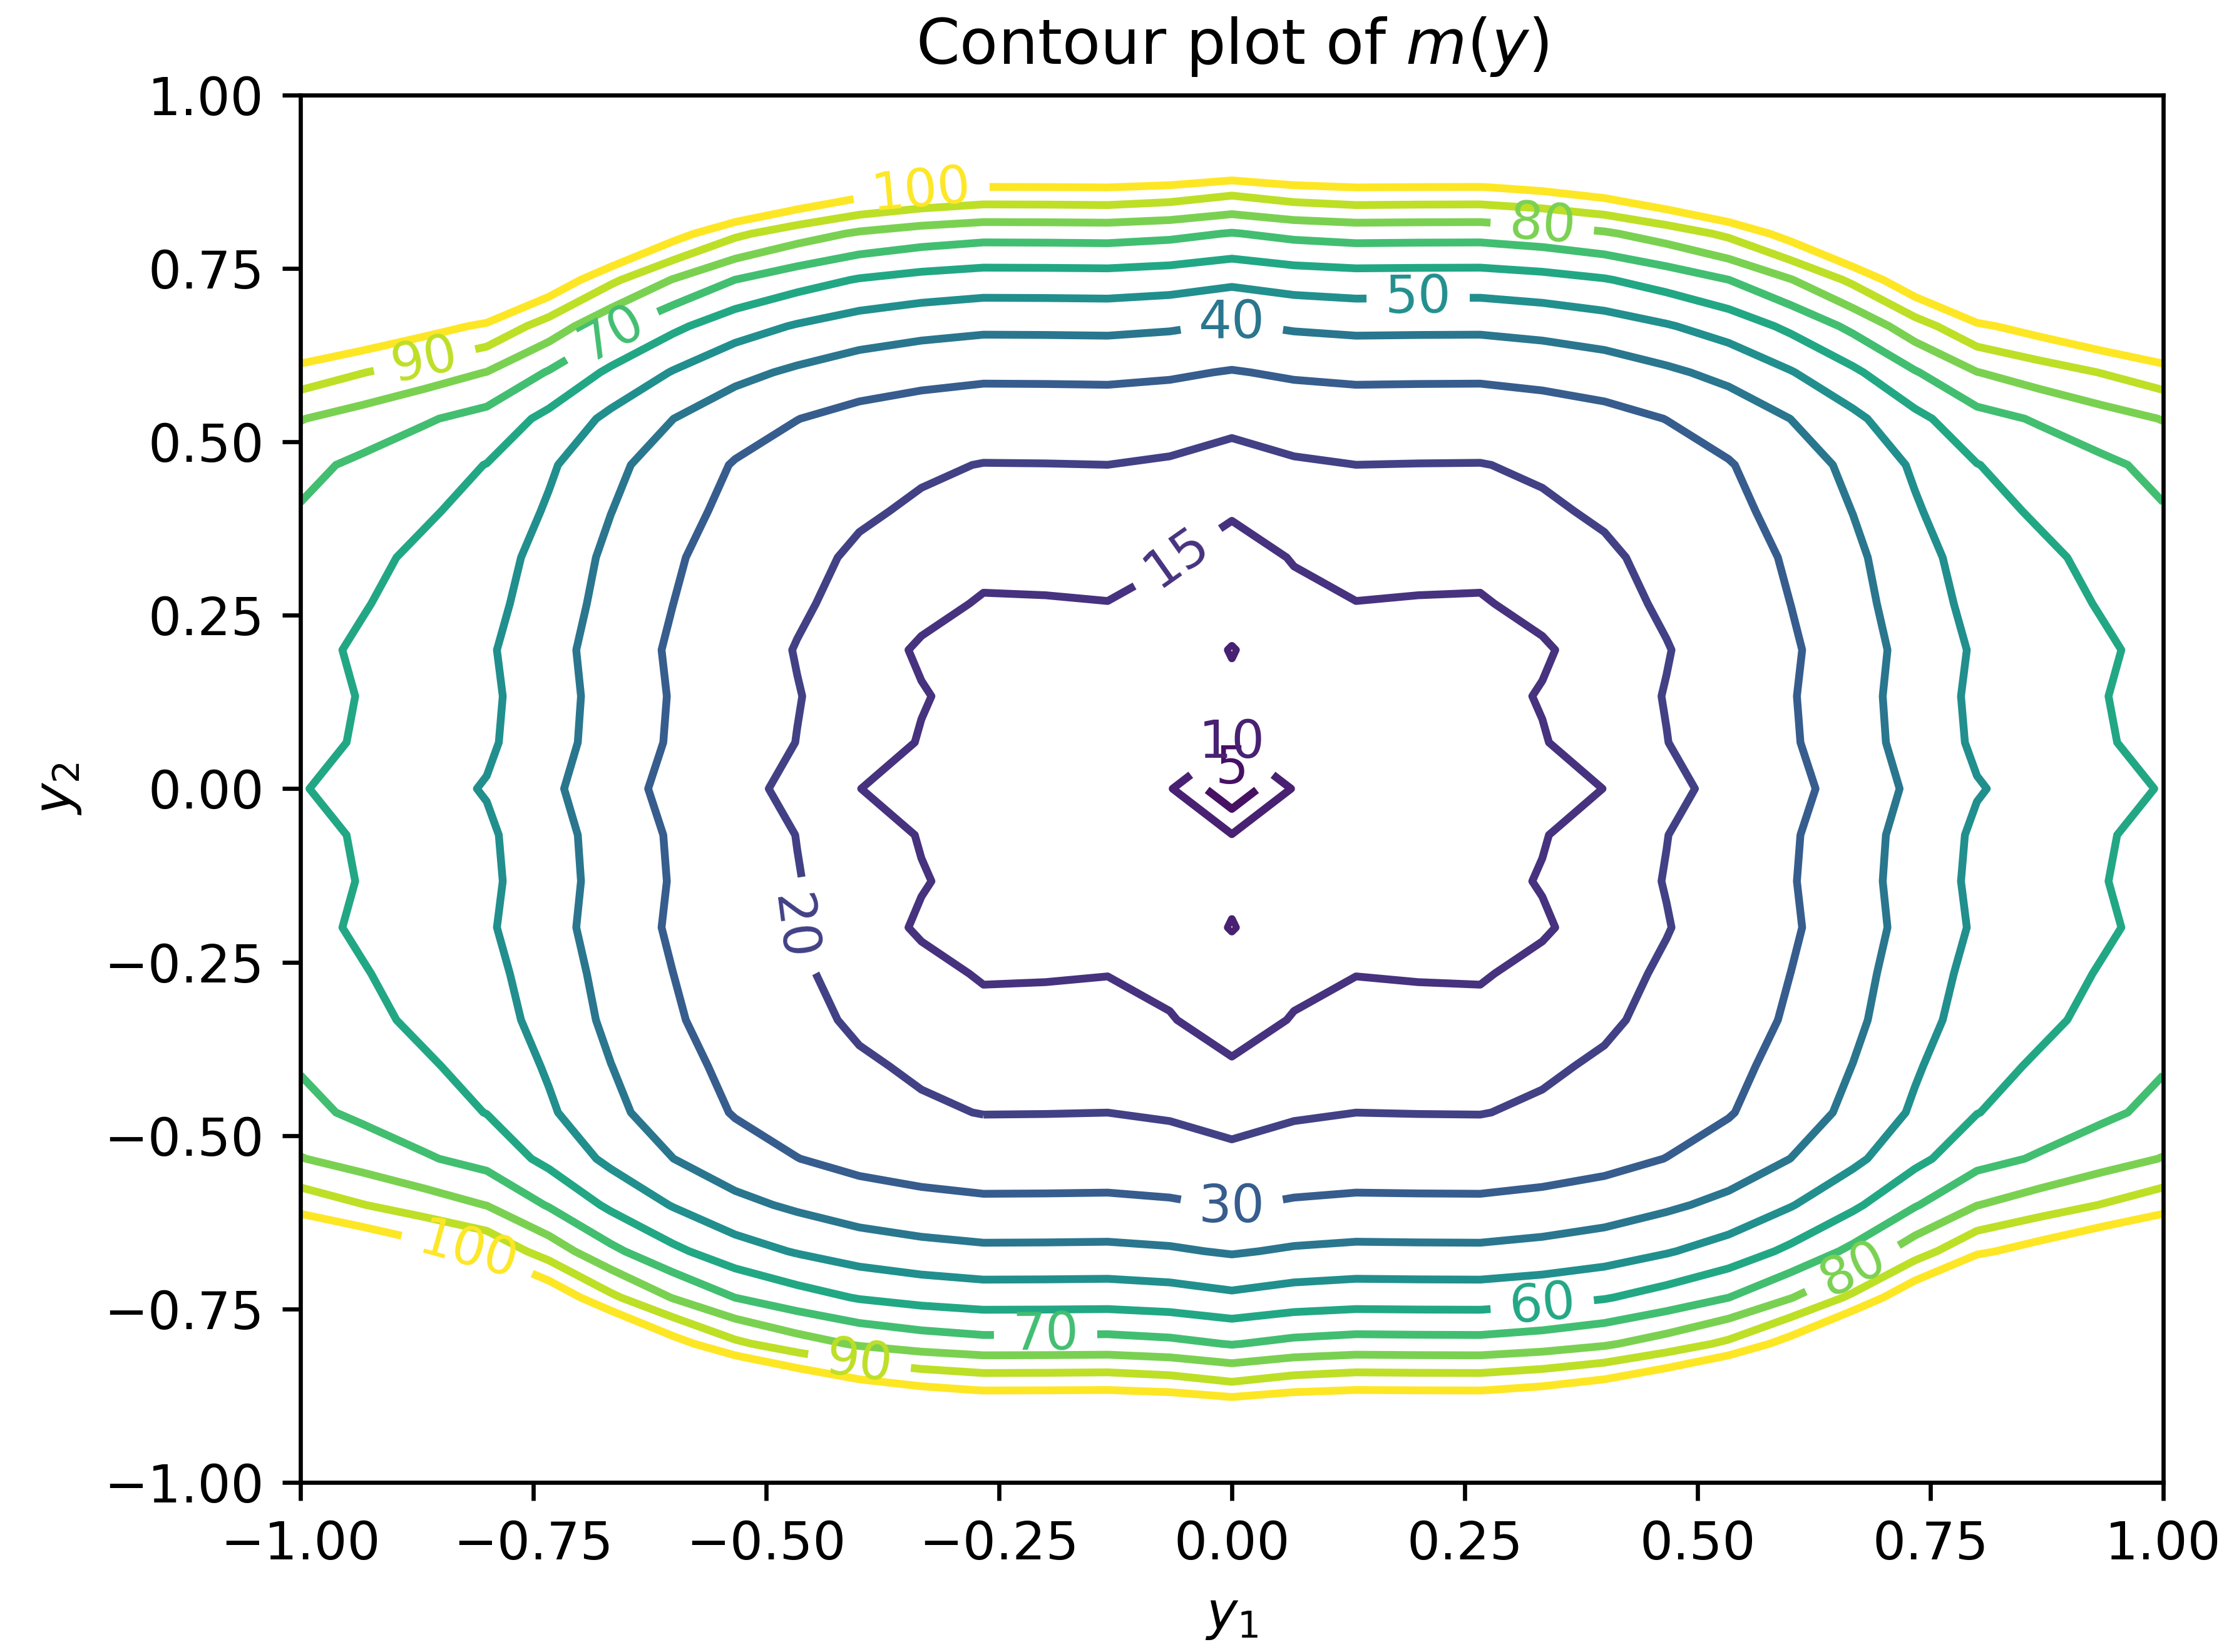
\includegraphics[width=\linewidth]{6-chapter/figures/contour2}
        \caption{} \label{fig:1b}
    \end{subfigure}%
%    \vspace*{-15pt}
    \caption{Result of the location-allocation algorithm; Figure~\ref{fig:1a} shows the preconditioner attributions together with the underlying partition of $W$, and Figure~\ref{fig:1b} shows a contour plot of the underlying distance function $m(\cdot)$.}
    \label{fig:voronoi_diagram}
\end{figure}

\subsection{Number of preconditioners}\label{subsec:Npc_experiment}
Figures~\ref{fig:Npc_tikz_2_5_10} and~\ref{fig:Npc_tikz_15_20_25} show the efficacy of the preconditioner count selection in Algorithm~\ref{alg:location-allocation}, for different parameter dimensions.
As discussed in Section~\ref{subsec:determining-Npc}, we re-use the initialization approach for efficiency.
To compare against the optimal choice, we perform greedy initialization and execute Algorithm~\ref{alg:location-allocation} after each step instead.
This allows us to check whether our approach is close to the optimal choice for $N_{pc}$.
We perform this comparison for the parameterized shape problem with parameter dimension $N=15$.

The red line in Figures~\ref{fig:Npc_tikz_2_5_10} and~\ref{fig:Npc_tikz_15_20_25} represents the greedy initialization costs, and the blue lines correspond to the costs after the location-allocation are steps taken as long as it is worth the computation time.
As expected, there is an optimal number of preconditioners, as the curves exhibit a minimum.
The red line being above the blue line indicates that the location-allocation procedure improves preconditioner placement.
The black curve shows results if we run location-allocation until full convergence.
Since it mostly overlaps with the blue, cutting location-allocation short has little impact, and our strategy is essentially optimal.

Focussing on the $N=15$ case at the bottom of Figure~\ref{fig:Npc_tikz_2_5_10}, we observe that the first half of the black and blue curves are a bit volatile, which we would not expect for the global optimum.
This volatility occurs because the location-allocation heuristic ends up in local minima, as we discussed back in Section~\ref{subsec:location}.
Interestingly, other tests that we performed showed that this volatility disappears for both small ($N \leq 5$) and large ($N \geq 25$) values of the parameter dimension.
Finally, we see the three curves converging for large values for $N_{pc}$, which indicates that the greedy initialization performs quite well whenever $\frac{|W|}{N_{pc}}$ is small.

For this run with parameter dimension $N=15$, the chosen value for $N_{pc}$ is at $N_{pc}^*=35$, marked by a vertical line in Figure~\ref{fig:Npc_tikz_2_5_10}.
This is lower than the minimum from the greedy initialization, which happened around $N_{pc}\approx 45$.
Still, the final strategy remains close to optimal.
Variance from local minima overshadows further improvements, making this a cost-effective method.

\begin{figure}
    \centering
    \vspace{-20pt}
    \begin{subfigure}[b]{\textwidth}
        \npcgraph{6-chapter/data/Npc22may/Npc_data_2.dat}
    \end{subfigure}
    \begin{subfigure}[b]{\textwidth}
        \vspace{-20pt}
        \npcgraph{6-chapter/data/Npc22may/Npc_data_5.dat}
    \end{subfigure}
    \begin{subfigure}[b]{\textwidth}
        \vspace{-20pt}
        \npcgraph{6-chapter/data/Npc22may/Npc_data_10.dat}
    \end{subfigure}
    \caption{
        Effect of different $N_{pc}$ values for the parameterized shape problem in parameter dimensions $N=2$ (top), $N=5$ (middle), and $N=10$ (bottom).
        The red curve shows the greedy initialization, the blue curve is the location-allocation result from Algorithm~\ref{alg:location-allocation}, and the black dashed curve is the result of the location-allocation algorithm until convergence.
        $N_{pc}^*$ is the value where Algorithm~\ref{alg:location-allocation} terminates.
    }
    \label{fig:Npc_tikz_2_5_10}
\end{figure}

\begin{figure}
    \centering
    \vspace{-20pt}
    \begin{subfigure}[b]{\textwidth}
        \npcgraph{6-chapter/data/Npc22may/Npc_data_15.dat}
    \end{subfigure}
    \begin{subfigure}[b]{\textwidth}
        \vspace{-20pt}
        \npcgraph{6-chapter/data/Npc22may/Npc_data_20.dat}
    \end{subfigure}
    \begin{subfigure}[b]{\textwidth}
        \vspace{-20pt}
        \npcgraph{6-chapter/data/Npc22may/Npc_data_25.dat}
    \end{subfigure}
    \caption{
        Effect of different $N_{pc}$ values for the parameterized shape problem in parameter dimensions $N=15$ (top), $N=20$ (middle), and $N=25$ (bottom).
        The red curve shows the greedy initialization, the blue curve is the location-allocation result from Algorithm~\ref{alg:location-allocation}, and the black dashed curve is the result of the location-allocation algorithm until convergence.
        $N_{pc}^*$ is the value where Algorithm~\ref{alg:location-allocation} terminates.
    }
    \label{fig:Npc_tikz_15_20_25}
\end{figure}

\subsection{Convergence of the surrogate model}\label{subsec:gpr_reliability_experiment}
The reliability of our preconditioning strategy hinges on a good estimation $m(\cdot)$ for the number of GMRES iterations, which we will explore in this section by using the parametric domain problem with parameter dimension $N=15$.
The results are shown in Figure~\ref{fig:surrogate_convergence2}.

We expect $m(\cdot)$ to predict iterations more accurately with more training data.
To verify this, we train the GPR with different numbers of training data $N_{train}$.
After each training point we add, we compute the root-mean-square error of $m(\cdot)$ over the domain $\{\y \in Y | m(\y) < N_{ratio} / 2\}$ using a Monte Carlo estimate.
This domain is taken such that we measure the accuracy of the surrogate over the relevant subset of the parameter space, as a parameter value with $m(\y)>\frac{N_{ratio}}{2}$ will most likely get assigned to another preconditioner even further from the origin.
We use a parameter dimension of $N=15$, anisotropy $\alpha=2$, and shape variation $\vartheta=\frac{1}{2}\vartheta_{\max}(\alpha=2)$.

Figure~\ref{fig:surrogate_convergence2} shows that the surrogate accuracy improves with more training data but plateaus at a saturation point.
Additionally, we observe that the disagreement ratio fluctuates significantly, highlighting the need for smoothing in the stopping criterion.
Once smoothened, the disagree ratio decays as we add more training data, and it crosses the $1\%$ threshold before reaching the saturation threshold.
We observe this behavior consistently across multiple runs and varying parameter dimensions, although the exact stopping point varies.
Despite the aggressiveness of the stopping criterion, the surrogate still enables the effective placement of preconditioners.

Finally, the RMSE converges to a value of approximately 3.
This value reflects the modeling error between the actual number of GMRES iterations needed and our surrogate $m(\cdot)$.
This originates from our kernel choice, where we assumed a dimensional splitting and symmetry around the origin from our kernel choice in equation~\eqref{eq:univariatekernel}.
These assumptions reduce accuracy but mitigate the curse of dimensionality.
A RMSE of 3 is still very acceptable, and the gained computational improvements are well worth it.
\begin{figure}
    \centering
    \begin{tikzpicture}
        \begin{axis}[
%            ymode=log,
            label style={font=\small},
            ticklabel style = {font=\small},
            axis y line=left,
            ymax=12,
            xmin=0,
            xmax=200,
            ytick={10, 8, 6, 4, 2},
            yticklabels={10, 8, 6, 4, 2},
            width=0.90\textwidth,
            height=0.45\textwidth,
            ylabel near ticks,
            legend columns=4,
            ylabel=RMSE]
            \addplot[black,thick] table [mark=none, x=Ntrain, y=Dimsum15]{6-chapter/data/LOOCV/SP05_bucket1.dat};
            \label{plot_one}
        \end{axis}
        \begin{axis}[
            axis y line=right,
            axis x line=none,
            ytick={1, 0.1, 0.01, 0.001, 0.0001},
            ymode=log,
            legend style={font=\fontsize{8}{7}\selectfont},
            label style={font=\small},
            ticklabel style = {font=\small},
            ymax=12,
            xmin=0,
%            grid=both,
            xmax=200,
            width=0.90\textwidth,
            height=0.45\textwidth,
            legend columns=2,
            ylabel=disagree ratio]

            \addlegendimage{/pgfplots/refstyle=plot_one}\addlegendentry{RMSE}
            \addplot[black,thick,dashed] table [mark=none, x=Ntrain, y=SP15]{6-chapter/data/LOOCV/SP05_bucket1.dat};
            \addlegendentry{disagree ratio}
            \addplot[black,thick,densely dotted, line width=1pt, color=red] table [mark=none, x=Ntrain, y=Smooth15]{6-chapter/data/LOOCV/SP05_bucket1.dat};
            \addlegendentry{smooth disagree ratio}
            \addplot[color=gray, line width=1pt] coordinates {(0, 0.01) (200, 0.01)};
            \addlegendentry{$1\%$}
        \end{axis}
    \end{tikzpicture}
    \caption{Comparison of the RMSE and disagree ratio for the stabilizing predictions (SP) stopping criterion.
    The parameter dimension is $N=15$ with $\vartheta=\frac{1}{2}\vartheta_{\max}$ and $\alpha=2$.
    The solid line represents the RMSE (left axis), the dashed line the disagree ratio, and the dotted line a trailing average of the disagree ratio (right axis).
    The solid gray line marks the $1\%$ threshold in the stopping criterion.
    }
    \label{fig:surrogate_convergence2}
\end{figure}
%\afterpage{\clearpage}
\subsection{Kernel comparison}\label{subsec:kernel-comparison}
In Chapter~\ref{ch:distributed-preconditioning}, we have introduced the kernel~\eqref{eq:sumkernel}, which is based on univariate kernels, where each univariate kernel consists of a symmetrized Matérn kernel.
Naturally, we ask ourselves how this choice compares against other kernels.
Therefore, we perform the training procedure for the parameterized scatterer problem for different kernels.
We train each kernel on the same sample set $W$, but we select the training points separately.
In this experiment, we consider the Matérn kernel, a symmetrized Matérn kernel, and the univariate Matérn kernel as in~\eqref{eq:sumkernel}.
To maximize the effect of the parameter dimension, we set $\alpha=2$ and $\vartheta = \vartheta_{\max}(\alpha=2)$.

Figures~\ref{fig:surrogate_convergence_kernels2-5-10} and~\ref{fig:surrogate_convergence_kernels15-20-25} show the results of these experiments.
From these figures, we can make several observations.
First, we observe that the symmetric Matérn and the univariate kernel in~\eqref{eq:sumkernel} do not exhibit significant differences in two parameter dimensions.
This is primarily due to the low dimensionality, which is confirmed when examining higher parameter dimensions.
For example, for $N=20$, we see a clear difference between the symmetric Matérn and univariate kernels, where the univariate kernel converges faster than the symmetric Matérn kernel.

For all parameter dimensions, the Matérn kernel converges the slowest.
This follows expectations, as the Matérn kernel represents a richer function space, requiring more training points to converge.
On the other hand, the Matérn kernel achieves lower RMSE values, also due to its richer function space.
This effect is most pronounced for lower parameter dimensions in Figure~\ref{fig:surrogate_convergence_kernels2-5-10}.

\begin{figure}
    \centering
    \begin{subfigure}[b]{\textwidth}
        \vspace{-5pt}
        \kernelplot{2}
    \end{subfigure}
    \begin{subfigure}[b]{\textwidth}
        \vspace{-5pt}
        \kernelplot{5}
    \end{subfigure}
    \begin{subfigure}[b]{\textwidth}
        \vspace{-5pt}
        \kernelplot{10}
    \end{subfigure}
    \caption{Averaged convergence graphs of the training procedure for parameter dimension $N=2$ (top), $N=5$ (middle), and $N=10$ (bottom) for different choices for the kernel in the GPR surrogate model $m(\cdot)$. }\label{fig:surrogate_convergence_kernels2-5-10}
\end{figure}

\begin{figure}
    \centering
    \begin{subfigure}[b]{\textwidth}
        \vspace{-5pt}
        \kernelplot{15}
    \end{subfigure}
    \begin{subfigure}[b]{\textwidth}
        \vspace{-5pt}
        \kernelplot{20}
    \end{subfigure}
    \begin{subfigure}[b]{\textwidth}
        \vspace{-5pt}
        \kernelplot{25}
    \end{subfigure}
    \caption{Averaged convergence graphs of the training procedure for parameter dimension $N=15$ (top), $N=20$ (middle), and $N=25$ (bottom) for different choices for the kernel in the GPR surrogate model $m(\cdot)$.}\label{fig:surrogate_convergence_kernels15-20-25}
\end{figure}